\documentclass[10pt,conference,compsocconf]{IEEEtran}

\usepackage{hyperref}
\usepackage{graphicx}	% For figure environment
\usepackage{amsmath}
\usepackage{amssymb}
\usepackage{float}


\begin{document}
\title{CS-433 Machine Learning Project 1}

\author{
  Matthias Minder, Zora Oswald, Silvan Stettler\\
  
}

\maketitle

\begin{abstract}
%%% abstract here
\end{abstract}

\section*{Introduction}
Collision events in the Large Hadron Collider at CERN do not create directly observable results. An essential part of elementary particles such as the Higgs boson therefore rely on classifying the collisions based on a number of variables that can be measured in the collider. 
In our dataset, a vector containing 30 dimensions describes one collision event. A binary classification algorithm can be used to predict the presence of a Higgs boson based on this feature vector. The model is trained with data from collisons for which the existence of a Higgs boson is determined.
Our classifications of the collision events consist of three main steps:
\begin{enumerate}
\item Imputation of missing data and normalization
\item Mapping of the input to a feature space with a non-linear kernel
\item Cross-validation of the binary classification methods
\item Application of the best-fitting binary model and corresponding hyper parameter to the test data
\end{enumerate}
\section*{Methods}
The raw dataset contains a significant amount of missing data. Thus, the first step consisted of imputing the missing features with reasonable values. Analysis of the raw data showed that there are a total of six different patterns of missing features. A pattern is characterized by a certain set of values missing in dimensions $M$ and values being present in dimensions $M'$ ($M+M' = 30$). For each pattern, a simple linear regression was fitted using the least-squares method with gradient descent, using the complete feature vectors $\boldsymbol{x_i}$ as training data. The optimized weight vector was then applied to the all the vectors with the same pattern of missing features $\boldsymbol{x}_{na,i}$ in order to predict the missing values.
\begin{align*}
{x}_{ij, j \in M} &\approx w_0 + \sum_{k \in M'} w_k {x}_{ik}\\
\boldsymbol{w}^* = \underset{x}{argmin}\sum_i & ({x}_{ij, j \in M} - \boldsymbol{x}^T_{ik, k \in M'} \boldsymbol{w})^2\\
{x}_{na,ij, j \in M} &= w_0 + \sum_{k \in M'} w_k {x}_{na,ik}
\end{align*} \par
Classifying the collision events comes down to finding a relationship between the continuous and independent inputs and a binary output describing the presence or absence of a Higgs boson. As seen in class, logistic regression lends itself well to this task and was thus the first model that we tested. 
The probability that a Higgs boson is present is given by the sigmoid function
\begin{align*}
\sigma(z) &= \frac{1}{1+e^{-z}} \in [0,1]\\
z & = \boldsymbol{Xw} 
\end{align*}
For values $\in (0.5,1]$, the collision is classified to have yielded a Higgs boson and assigned the label $1$. For values below $0.5$, the label $0$ is assigned respectively. A $L_2$-regularized cost function was used in order to avoid that the weight vector $\boldsymbol{w}$ tends to infinity.  
\begin{equation}
\mathcal{L}(\boldsymbol{w}) = \sum_{n=1}^N ln(1+e^{\boldsymbol{x}^T\boldsymbol{w}}) - y_n \boldsymbol{x}^T\boldsymbol{w} + \frac{\lambda}{2}||\boldsymbol{w}||^2
\end{equation}
The above cost function was minimized using the stochastic gradient method. \par
The feature vector $\boldsymbol{X}$ in the above equations contains a constant term. In addition, the influence of enhancing the feature vector with the squares of each value was assessed. This enhanced feature vector has the form
\begin{equation}
\boldsymbol{x}_{enh.} = [1 \hspace{2mm} \boldsymbol{x}_n \hspace{2mm} \boldsymbol{x}_n^2]
\end{equation}

%%% TODO: SVM description

\section*{Results}
The hyper-parameter $\lambda$ was tuned to minimize the number of misclassified collision events using the $K$-fold cross validation technique, where $K$ was chosen to be 10
\begin{figure}[H]
	\centering
	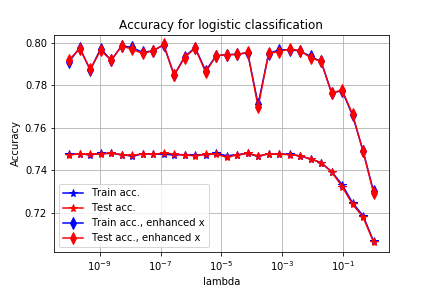
\includegraphics[width=0.45\textwidth]{accuracy_logistic.png}
	\caption{10000 iterations, $\gamma$ = 0.001}
\end{figure}

%%% TODO: same for SVM

\section*{Conclusion}

%%% Bibliography
\bibliographystyle{IEEEtran}
\bibliography{literature-project1}

\end{document}